\newpage

\section{Diagrama de sequência}

A realização da autenticação, ativação e confirmação da conta requerem procedimentos extras e seguem determinadas regras. Deste modo, foi necessário elaborar diagramas de sequência para especificar as interações com o sistema.

\subsection{Diagrama de sequência Login e ativação de conta}

O objetivo do diagrama da figura~\ref{fig:43} consiste em demonstrar, que assim que o técnico realiza o login, é necessário verificar as credenciais. Se estas estiverem incorretas, este receberá uma mensagem de erro. Contudo, caso estas estejam válidas e a conta estiver ativada o técnico ficará autenticado. 

Se porventura o técnico colocar as credenciais corretas, mas a conta não estiver ativada, este irá realizar a ativação da conta, onde poderá enviar o código de ativação. Se eventualmente estiver correto, a conta será ativada, caso contrário, este receberá uma mensagem de erro. Porém, o técnico também terá como hipótese cancelar a ativação da conta e/ou pedir um novo \textit{email} de ativação, onde será pedido um novo código ao servidor e este automáticamente será gerado e enviado.

\begin{figure}[htb]
    \centering
    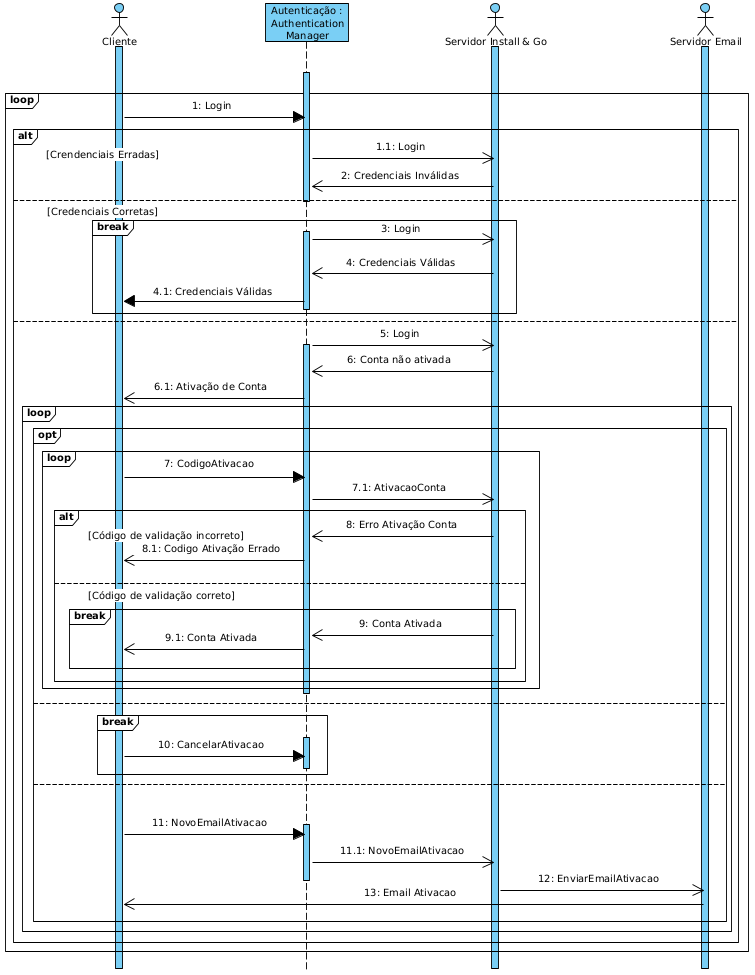
\includegraphics[width=0.64\textwidth]{images/diagramas/sequencia/diagrama_login.png}
    \caption{Diagrama de sequência de login e ativação de conta}
    \label{fig:43}
\end{figure}

\newpage

\subsection{Diagrama de sequência Registo e ativação de conta}

Através do diagrama da figura~\ref{fig:44} é possível perceber que quando uma empresa realiza o registo, este será enviado para o servidor, o qual registará a empresa com uma conta não ativada. Esta conta será validada pela Motorline, de seguida é gerado um código de ativação e por fim é enviado para o \textit{email} de registo. Após o registo ou o clique em ativar a conta no \textit{email} recebido, a empresa será encaminhada para a validação de conta e toda a validação ocorre conforme o processo mencionado no anteriormente.

\begin{figure}[htb]
    \centering
    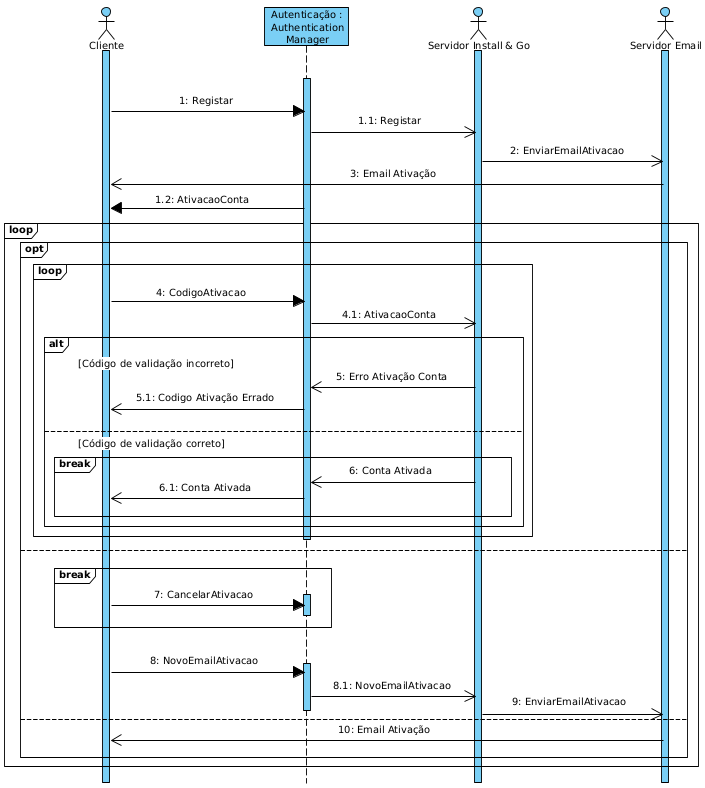
\includegraphics[width=\textwidth]{images/diagramas/sequencia/diagrama_registo.png}
    \caption{Diagrama de sequência de registo e validação de conta}
    \label{fig:44}
\end{figure}

\newpage

\subsection{Diagrama de sequência registo de técnicos}

O diagrama da figura~\ref{fig:45} tem como propósito dar a perceber que quando uma empresa deseja registar um técnico esta introduzirá os seus dados no sistema, o que leva estes a serem enviados e a conta criada. Posteriormente, um código de ativação é gerado e enviado para o técnico poder ativar a sua conta, este processo segue a mesma orientação mencionada anteriormente.

\begin{figure}[htb]
    \centering
    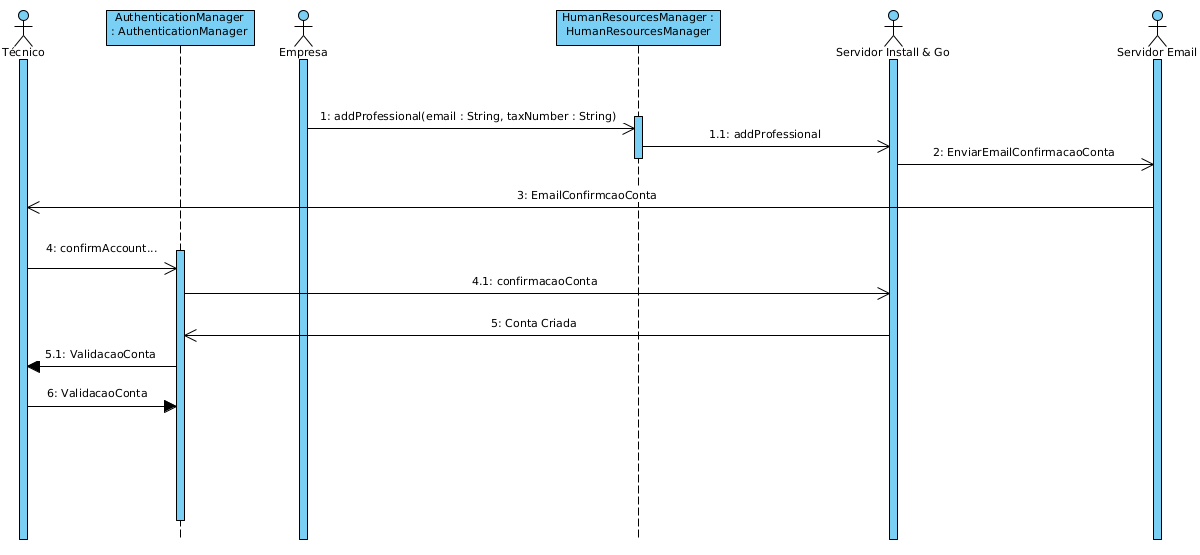
\includegraphics[width=\textwidth]{images/diagramas/sequencia/registo_tecnico.png}
    \caption{Diagrama de sequência de registo de técnicos}
    \label{fig:45}
\end{figure}